\documentclass[a4paper,12pt]{article} % Classe du document
%--------------------- Packages ------------------------

\RequirePackage[french]{babel} %Langue du document
\RequirePackage[utf8]{inputenc} %Caractères spéciaux
\RequirePackage[section]{placeins}%Pour placement de section
\RequirePackage[T1]{fontenc} %Quelques lettres qui sont pas inclus dans UTF-8
\RequirePackage{mathtools} %Paquet pour des équations et symboles mathématiques
\RequirePackage{siunitx} %Pour écrire avec la notation scientifique (Ex.: \num{2e+9})
\RequirePackage{float} %Pour placement d'images
\RequirePackage{graphicx} %Paquet pour insérer des images
\RequirePackage[justification=centering]{caption} %Pour les légendes centralisées
\RequirePackage{subcaption}
\RequirePackage{wallpaper}
\RequirePackage{nomencl}
\makenomenclature
\RequirePackage{fancyhdr}
\pagestyle{fancy}
\fancyheadoffset{1cm}
\setlength{\headheight}{2cm}
\setlength{\parindent}{0cm} 
\RequirePackage{url}
\RequirePackage[hidelinks]{hyperref}%Paquet pour insérer légendes dans des sous-figures comme Figure 1a, 1b
\RequirePackage[left=2.5cm,right=2.5cm,top=2cm,bottom=3.5cm]{geometry} %Configuration de la page

\usepackage{pythontex}%pour utiliser python

%-------------------- Informations sur le rapport ----------------------

\newcommand{\nom}[1]{\renewcommand{\nom}{#1}}

\begin{document}

%----------- Informations du rapport ---------

\nom{Prénom NOM}

%----------- Initialisation -------------------
  
\lhead{\nom} %Header Left
%\chead{} %Header center
\rhead{\nouppercase{\today}} %Header right
\rfoot{\thepage} %Footer right
\cfoot{titre} %Footer center
\lfoot{titre secondaire} %Footer left

\begin{titlepage}
    %créer la page de garde ici
     \centering   
        \vfill
        {\large \today\par} %Affichage de la date
    
    \end{titlepage}
\tableofcontents %Créer la table de matières
\newpage 

%------------ Corps du rapport ----------------
%------------- Commandes utiles ----------------

\section{Quelques commandes}

Voici quelques commandes utiles :

\subsection{Image}
%------ Pour insérer et citer une image centralisée -----

\begin{figure}[H] %le H sert à fixer l'image à cette endroit dans le texte
    \center
    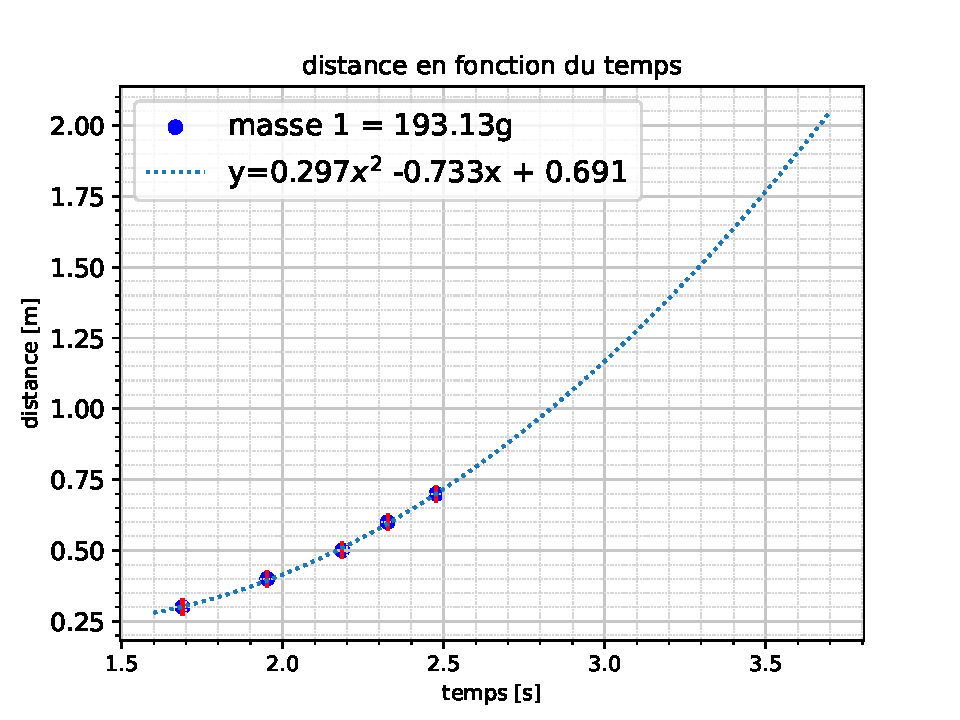
\includegraphics[width=16cm]{./logos/graph.pdf}
    \caption{Graphique}
    \label{Label de la figure}
\end{figure}

Ici, je cite l'image \ref{Label de la figure}.

\subsection{Équation}

%------- Pour insérer et citer une équation --------------

\begin{equation} \label{eq: exemple}
\rho + \Delta = 42
\end{equation}

L'équation \ref{eq: exemple} est cité ici. 

\subsection{Pythontex}
% ------- Pour écrire des variables ----------------------

Pour écrire des variables dans le texte, il suffit de mettre le symbole \$ entre le texte souhaité comme : constante $\rho$.

Pour utiliser pythontex :
\begin{pycode}
x = 3 #attention à l'indentation, il ne doit pas y avoir d'espaces avant la ligne
\end{pycode}
       
$x = \py{x}$

si x = ?? effectuer :
pythontex main.tex

Il est aussi possible d'écrire le code python dans autre fichier .tex
et l'inclure dans ce fichier.
\begin{pycode}
a = 23
b=4.23
c=2.2
d=3
e=0.3456
tableau_calc = '\\begin{tabular}{|c|c|c|c|c|}\n'
tableau_calc += '\\hline\n'
tableau_calc += '$a_1$ & $b_{test}$ & $c$ & d & $e$  \\\\ \\hline\n'
tableau_calc += f'{a} & {b} & {c} & {d} & {e} $m/s^2$\\\\ \\hline\n'
tableau_calc += '\\end{tabular}\n'
\end{pycode}

On peut aussi créer des tableaux latex en code python :

\begin{figure}[H]
    \centering
    \py{tableau_calc}
\end{figure}

Si il y a une erreur de compilation à cause du tableau,
comme celle-ci : Missing \$ inserted.

Supprimer le dossier pythontex-files-main et recompiler.

\subsection{Python}
Il peut être plus facile de créer des graphiques dans un fichier python séparé
et les sauvegarder comme images.

Un exemple de graphique (image \ref{Label de la figure}) a été crée avec python dans le dossier graph.  %pour inclure un autre fichier .tex

\end{document}
